% Based on Flowcharting techniques for easy maintenance by Brent Longborough
% https://texample.net/tikz/examples/flexible-flow-chart/

\documentclass[x11names,, border=20pt]{standalone}

\usepackage{tikz}
\usetikzlibrary{shapes,arrows,chains}
\begin{document}
% =================================================
% Set up a new layer for the debugging marks, and make sure it is on
% top
\pgfdeclarelayer{marx}
\pgfsetlayers{main,marx}
% A macro for marking coordinates (specific to the coordinate naming
% scheme used here). Swap the following 2 definitions to deactivate
% marks.
\providecommand{\cmark}[2][]{%
  \begin{pgfonlayer}{marx}
    \node [nmark] at (c#2#1) {#2};
  \end{pgfonlayer}{marx}
  } 
\providecommand{\cmark}[2][]{\relax} 
% -------------------------------------------------
% Start the picture
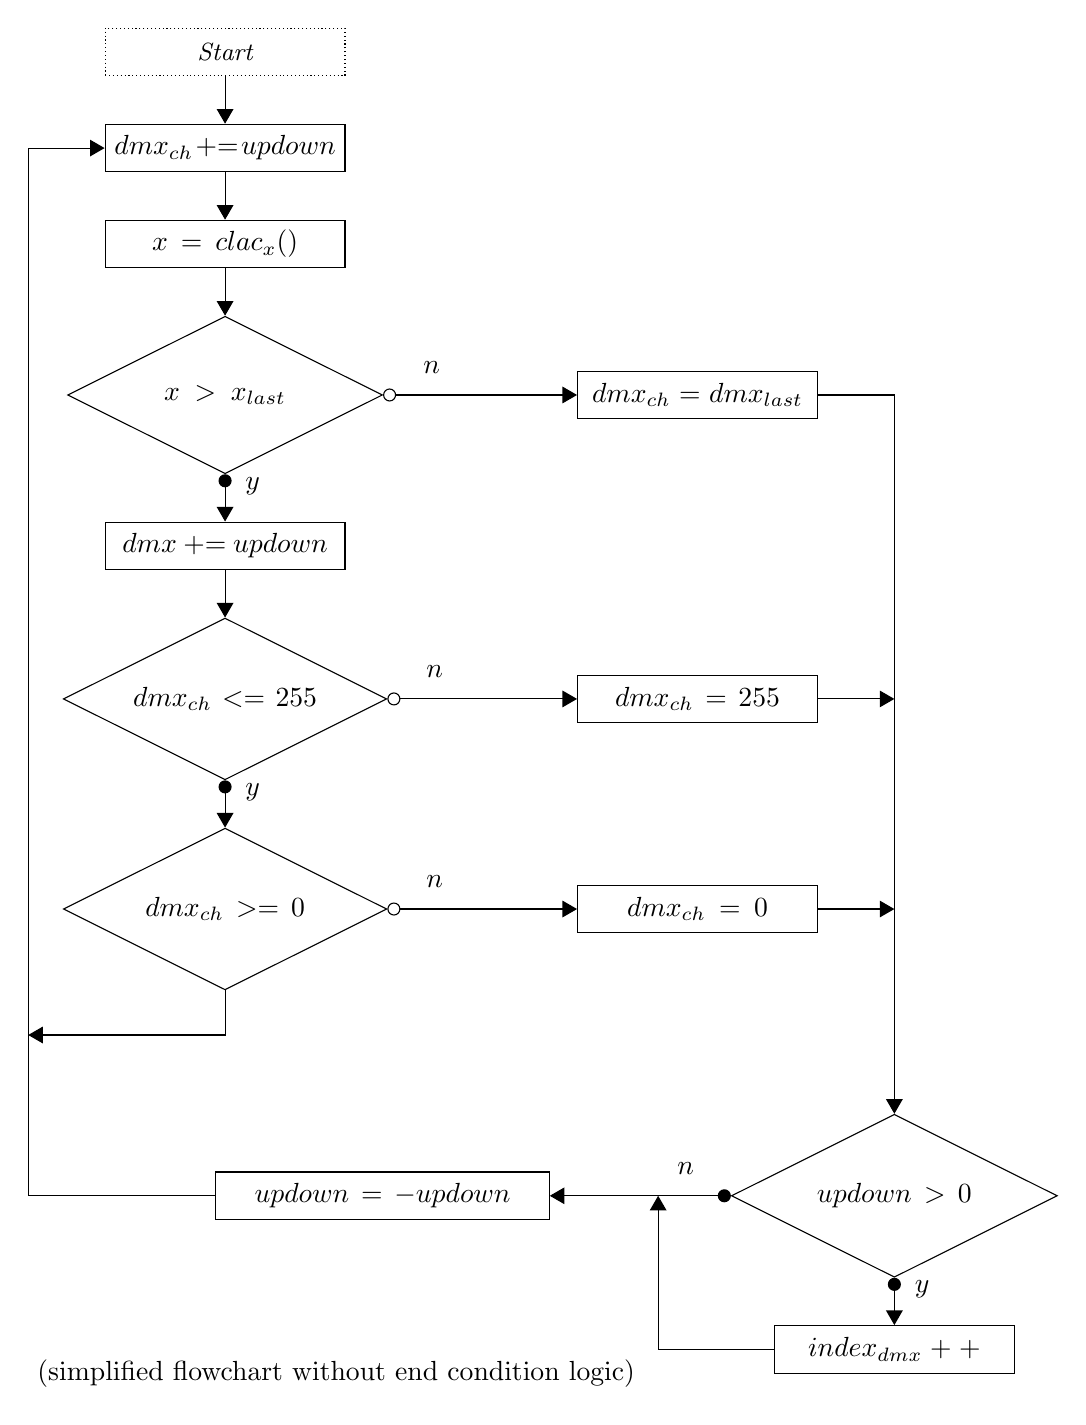
\begin{tikzpicture}[%
    >=triangle 60,              % Nice arrows; your taste may be different
    start chain=going below,    % General flow is top-to-bottom
    node distance=6mm and 60mm, % Global setup of box spacing
    every join/.style={norm},   % Default linetype for connecting boxes
    ]
% ------------------------------------------------- 
% A few box styles 
% <on chain> *and* <on grid> reduce the need for manual relative
% positioning of nodes
\tikzset{
  base/.style={draw, on chain, on grid, align=center, minimum height=4ex},
  proc/.style={base, rectangle, text width=8em},
  test/.style={base, diamond, aspect=2, text width=8em},
  term/.style={proc, rounded corners},
  % coord node style is used for placing corners of connecting lines
  coord/.style={coordinate, on chain, on grid, node distance=6mm and 25mm},
  % nmark node style is used for coordinate debugging marks
  nmark/.style={draw, cyan, circle, font={\sffamily\bfseries}},
  % -------------------------------------------------
  % Connector line styles for different parts of the diagram
  norm/.style={->, draw},
  free/.style={->, draw, lcfree},
  cong/.style={->, draw, lccong},
  it/.style={font={\small\itshape}}
}
% -------------------------------------------------
% Start by placing the nodes
\node [proc, densely dotted, it] (p0) {Start};
% Use join to connect a node to the previous one 
% No join for exits from test nodes - connections have more complex
% requirements
% We continue until all the blocks are positioned
\node [proc, join] (p2) {$dmx_{ch} \mathbin{{+}{=}} updown$};
\node [proc, join] (cx) {$x=clac_x()$};
\node [test, join] (xx) {$x>x_{last}$};
\node [proc] (updown) {$dmx \mathbin{{+}{=}} updown$};
\node [test, join] (dmx255) {$dmx_{ch}<=255$};
\node [test] (dmx0) {$dmx_{ch}>=0$};

% We position the next block explicitly as the first block in the
% second column.  The chain 'comes along with us'. The distance
% between columns has already been defined, so we don't need to
% specify it.

\node [proc, right=of xx] (pxx) {$dmx_{ch}=dmx_{last}$};
% Some more nodes specifically positioned (we could have avoided this,
% but try it and you'll see the result is ugly).
\node [proc, right=of dmx255] (p255) {$dmx_{ch}=255$};
\node [proc, right=of dmx0] (p0) {$dmx_{ch}=0$};
% -------------------------------------------------
% Now we place the coordinate nodes for the connectors with angles, or
% with annotations. We also mark them for debugging.  
\node [coord, below=of dmx0, yshift=-10mm, xshift=-25mm] (cfin)  {};% \cmark{fin}
\node [coord, right=of p255] (c255)  {}; %\cmark{255}
\node [coord, right=of p0] (c0)  {}; %\cmark{0}
\node [coord, right=of pxx] (cxx)  {};% \cmark{xx}  

\node [test, below=of c0, yshift=-20mm] (first) {$updown>0$};
\node [proc] (pipp) {$index_{dmx}++$};
\node [proc, left=of first, text  width=4cm, xshift=-5mm] (puu) {$updown=-updown$};

\node [coord, left=of first, xshift=-5mm] (cuu)  {}; %\cmark{uu}  
% -------------------------------------------------
% A couple of boxes have annotations

% -------------------------------------------------
% All the other connections come out of tests and need annotating
% First, the straight north-south connections. In each case, we first
% draw a path with a (consistently positioned) annotation node, then
% we draw the arrow itself.
\path (xx.south) to node [near start, xshift=1em] {$y$} (updown);
\draw [*->] (xx.south) -- (updown);
\path (dmx255.south) to node [near start, xshift=1em] {$y$} (dmx0);
\draw [*->] (dmx255.south) -- (dmx0);
\path (first.south) to node [near start, xshift=1em] {$y$} (pipp);
\draw [*->] (first.south) -- (pipp);
% ------------------------------------------------- 
% Now the straight east-west connections. To provide consistent
% positioning of the test exit annotations, we have positioned
% coordinates for the vertical part of the connectors. The annotation
% text is positioned on a path to the coordinate, and then the whole
% connector is drawn to its destination box.
\path (xx.east) to node [near start, yshift=1em] {$n$} (pxx); 
\draw [o->] (xx.east) -- (pxx);
\path (dmx255.east) to node [near start, yshift=1em] {$n$} (p255); 
\draw [o->] (dmx255.east) -- (p255);
\path (dmx0.east) to node [near start, yshift=1em] {$n$} (p0); 
\draw [o->] (dmx0.east) -- (p0);
\path (first.west) to node [near start, yshift=1em] {$n$} (puu);
\draw [*->] (first.west) -- (puu);
% -------------------------------------------------
% Finally, the twisty connectors. Again, we place the annotation
% first, then draw the connector
\draw [->] (pxx.east) -| (first);
\draw [->] (p255.east) -- (c255);
\draw [->] (p0.east)  -- (c0);
\draw [->] (pipp.west) -| (cuu);
% -------------------------------------------------
% A last flourish which breaks all the rules
\draw [->]
  (dmx0.south) |- (cfin);
\draw [->]
  (puu.west) -| (cfin)|-  (p2);
% -------------------------------------------------
\node[ right] at (current bounding box.south west){(simplified flowchart without end condition logic)};
\end{tikzpicture}
% =================================================
\end{document}